\documentclass[nonatbib]{elsarticle}
\makeatletter
\let\c@author\relax
\makeatother
% \usepackage{global-layout-notes}
\RequirePackage{amsmath, amssymb, amsthm, mathtools}
\newtheorem{theorem}{Theorem}
\RequirePackage{bm} 		% \bm for bold mathematical symbols
\RequirePackage{bbm} 		% \bm for bold mathematical symbols
\RequirePackage{xcolor}
\RequirePackage[colorlinks]{hyperref}
\RequirePackage{cleveref}
\RequirePackage[style=authoryear,backend=biber]{biblatex}
\bibliography{biblio}
\RequirePackage{statmacros}

\RequirePackage{import}
\RequirePackage{pdfpages}
\RequirePackage{transparent}
\RequirePackage{xcolor}

\newcommand{\incfig}[2][1]{%
    \def\svgwidth{#1\textwidth}
    \import{./figures/}{#2.pdf_tex}
}

\begin{document}
\title{Bayesian nonparametric multiscale mixture models via Hilbert-curve partitioning}
\author[add1]{Daniele Zago\corref{cor1}}
\ead{daniele.zago.1@studenti.unipd.it}
\author[add1,add2]{Marco Stefanucci}
\ead{stefanucci@stat.unipd.it}
\author[add1]{Antonio Canale}
\ead{canale@stat.unipd.it}


\cortext[cor1]{Corresponding author}

\address[add1]{Department of Statistical Sciences, University of Padova, Padova, Italy}
\address[add2]{Department of Economic, Business, Mathematical and Statistical Sciences, University of Trieste, Trieste, Italy}
\date{v0.1 on \today}

\begin{abstract}
    Bayesian nonparametric multivariate density estimation typically relies on mixture specifications, exceptions made for Pólya tree constructions. Herein, we develop a multivariate mixture model exploiting the multiscale stick-breaking prior recently proposed by \textcite{stefanucci2021}. The building block of the proposed approach is a base measure defined exploiting the Hilbert
    space-filling curve which allows to adapt a simple partitioning of a univariate parameter space to the multivariate case with minor adjustments. Alongside the theoretical discussion, we illustrate the model's performance by analyzing both synthetic and real datasets. The results suggest that the proposed multiscale model achieves competitive performance with respect to state-of-the-art Bayesian nonparametric methods both in scenarios presenting single- and multi-scale features.
\end{abstract}

\maketitle

\textbf{Keywords} Bayesian nonparametrics; multiscale models; density estimation; Dirichlet process; Pitman-Yor process

\section{Introduction}\label{sec:intro}
Nonparametric models typically characterize the unknown data distribution $F$ through an infinite-dimensional statistical model.
Bayesian nonparametric models (BNP) require the definition of a prior distribution over infinite-dimensional probability spaces in order to obtain an inferential procedure which is robust to model misspecifications.


\section{Multiscale mixture models}\label{sec:msmk}
Let $Y\in \mathcal{Y} \subseteq \R^{d}$ be a random variable.
We assume a multiscale representation for the density $f$ of $Y$,


\begin{equation}
    \label{eq:msMKprior}
    f(y) = \sum_{s=0}^{\infty }\sum_{h=1}^{2^{s}} \pi_{s,h} \mathcal{K}(y; \bm{\vartheta}_{s,h}),
\end{equation}
where $\mathcal{K}(\cdot ;\bm{\vartheta})$ is a kernel function defined on $\mathcal{Y}$ and parametrized by $\bm{\vartheta}$.
$\left\{ \pi_{s,h} \right\}$ is a sequence of mixture weights such that $\sum_{s=0}^{\infty }\sum_{h=1}^{2^{s}} \pi_{s,h} = 1$, and $\left\{ \bm{\vartheta}_{s,h} \right\} \subseteq \Theta$ is a sequence of kernel parameters.
This construction is reminiscent of the stick-breaking representation of the Dirichlet process mixture model \autocite{ferguson1983}, and it allows us to relate the representation of the density to an infinitely deep binary tree, whose nodes are indexed by a pair of indices $(s, h)$.
Thus, each node is uniquely identified by the set of parameters $\left\{ (\pi_{s,h},\bm{\vartheta}_{s,h})\right\}$.
\autoref{fig:btree} shows a truncation of such a binary tree at depth $s = 3$.



\begin{figure}[htbp]
    \centering
    % trim l b r u
    \fontsize{7pt}{8pt}\selectfont
    \incfig[1]{bintree}
    \caption{Binary tree representation of the mixture model, truncated at scale $s = 3$. At each node, $\bm{\vartheta}_{s,h}$ and $\pi_{s,h}$ are the associated kernel parameters and mixture weight, respectively.}
    \label{fig:btree}
\end{figure}


The density in \eqref{eq:msMKprior} can be equivalently rewritten as a Lebesgue integral of the kernel function with respect to a discrete mixing measure $P$,
\begin{equation}
    \label{eq:msMKpriorLebesgue}
    f(y) = \int \mathcal{K}(y; \bm{\vartheta}) \: dP(\bm{\vartheta}), \quad P = \sum_{s=0}^{\infty }\sum_{h=1}^{2^{s}} \pi_{s,h} \delta_{\bm{\vartheta}_{s,h}},
\end{equation}


where $\delta_{\bm{\vartheta}_0}$ denotes the Dirac delta function centered in $\bm{\vartheta} = \bm{\vartheta}_0$.\\


We can place a nonparametric prior distribution on $f$ by specifying a stochastic process that generates the mixing measure $P$ or, equivalently, the sequence of parameters $\left\{ (\pi_{s,h}, \bm{\vartheta}_{s,h}) \right\}$.
We will therefore begin the specification of this stochastic process by discussing the generation of the prior mixing weights $\left\{ \pi_{s,h} \right\}$.

\subsection{Mixture weights}\label{ssec:mixture-weights}
The sequence of mixture weights $\left\{ \pi_{s,h} \right\}$ is generated by the stochastic process introduced in \textcite{canale2016b}.
The construction closely resembles the stick-breaking construction of the Dirichlet process \autocite{sethuraman1994} and has been adapted in order to be employed in a binary tree setting.
More specifically, let $S_{s,h}$ and $R_{s,h}$ be random variables that take values in $(0,1)$.
$S_{s,h}$ denotes the probability of stopping at node $(s,h)$, whereas $R_{s,h}$ denotes the probability of taking the right path from node $(s,h)$ to node $(s+1, 2h)$, conditionally on not stopping on node $(s,h)$.
We also introduce an auxiliary variable $T_{shr}$ such that
\[
    T_{shr} = \begin{cases}
        R_{r, \left\lceil h 2^{r-s} \right\rceil } & \text{if } \left\lceil h 2^{r-2+1} \right\rceil = 2h\\

        1 - R_{r, \left\lceil h 2^{r-s} \right\rceil } & \text{otherwise}
    \end{cases}.
\]

The mixture weights are then defined as
\begin{equation}
    \label{eq:weightsStickBreaking}
    \pi_{s,h} = S_{s,h} \prod_{r < s} \big( 1 - S_{r, \left\lceil h 2^{r-s} \right\rceil } \big)T_{shr}.
\end{equation}


Equation \eqref{eq:weightsStickBreaking} describes a two-stage stick-breaking process that generates the mixture weights:
the stick of length one is initially broken according to the distribution of $S_{0,1}$, and its value is given to the first weight $\pi_{0,1}$.
The remainder of the stick, whose length is now $1 - S_{0,1}$, is then randomly split into two parts according to the distribution of $R_{0,1}$.
The two parts are then assigned to the children of the parent node, in this case $(1,1)$ and $(1,2)$, and the process is repeated.
The auxiliary variable $T_{shr}$ is useful to keep track of the differing stick lengths between the left and right children of each node.\\


The resulting algorithm allows us to generate all the mixture weights and guarantees that the sequence of weights $\left\{ \pi_{s,h} \right\}$ is such that \autocite{canale2016b}
\[
    \sum_{s=0}^{\infty }\sum_{h=1}^{2^{s}} \pi_{s,h} = 1 \quad \text{almost surely}.
\]



By way of analogy to the stick-breaking construction of \textcite{ishwaran2001}, the random variables $S_{s,h}$ and $R_{s,h}$ are given a prior distribution
\[
    S_{s,h} \sim \text{Beta}(a_s, b_s), \quad R_{s,h} \sim \text{Beta}(c_s, c_s),
\]


where the parameters $a_s, b_s, c_s$ define the behaviour of the weight-generating process.
This is similar to the way the behaviour of the Dirichlet process and its generalization, the Pitman-Yor process, depend on the choice of the parameters of the underlying Beta distribution.
Indeed, for $\delta \in [0,1) $ and $\alpha > -\delta$, we can choose the distributions
\begin{equation}
    \label{eq:betaStickBreaking}
    S_{s,h} \sim \text{Beta}\big(1 - \delta, \alpha + \delta(s+1)\big), \quad R_{s,h} \sim \text{Beta}(\beta,\beta),
\end{equation}
in order to mimic the stick-breaking representation of the Pitman-Yor process.
\textcite{stefanucci2021} provide an interpretation of the stick-breaking distributions in \eqref{eq:betaStickBreaking}, by observing that $\delta$ plays a similar role to the discount parameter $\sigma$ of the stick-breaking representation Pitman-Yor process.
In this case, $\delta$ controls the prior expected scale at which an observation falls, $\mathbb{E}\big[ \tilde{S} \big] = \sum_{s=0}^{\infty }s \mathbb{E}\big[ \pi_{s,h} \big]$.
More formally, we observe that the expected value of $S_{s,h}$ is heavily influenced by $\delta$, since
\[
    \mathbb{E}\big[ S_{s,h} \big] = \frac{1 - \delta}{\alpha + \delta(s+1)}.
\]
We can easily see that increasing $\delta$ results in a lower expected value for $S_{s,h}$; this, in turn means that the unitary stick is, on average, broken by smaller pieces at each scale.
Therefore, a larger value of $\delta$ favours \textit{a priori} deeper trees over shallower ones.
Following the discussion in \textcite{stefanucci2021}, we can numerically compute suitable values of $\alpha$ and $\delta$ in order to guarantee a desired prior expected tree depth $\mathbb{E}\big[ \tilde{S} \big].$

\subsection{Kernel parameters}\label{sec:kernel-parameters}
In this section we will present a multivariate generalization of the stochastic processes developed in \textcite{stefanucci2021} for mixtures of univariate kernels.
In their exposition, they consider a parameter space of the form $\Theta = \Theta_\mu \times \Theta_{\omega} \subseteq \R \times \R^+  $, so that $\left\{ \bm{\vartheta}_{s,h} \right\} = \left\{ (\mu_{s,h}, \omega_{s,h}) \right\} \subseteq \Theta$ is a sequence of location and scale parameters.
The resulting model is a mixture of univariate location and scale kernels $\mathcal{K}(\cdot ; \mu_{s,h}, \omega_{s,h})$, for which they provide a suitable stochastic process that generates each component separately.
We will now consider the multivariate generalization of this location and scale setting, where we denote by $\mathcal{K}(\cdot ; \bm{\mu}_{s,h}, \Omega_{s,h})$ the $d$-dimensional kernel defined on the sample space $\mathcal{Y}$.
In this case, the parameter space is $\Theta = \Theta_{\bm{\mu}} \times \Theta_{\Omega} \subseteq \R^{d} \times \mathcal{M}_{d}$, where $\mathcal{M}_{d}$ is the set of positive-definite square matrices of dimension $d\times d$.
In the general case, we are interested in constructing suitable stochastic processes to separately generate the sequence of location parameters $\left\{ \bm{\mu}_{s,h} \right\}$ and scale parameters $\left\{ \Omega_{s,h} \right\}$.

\subsubsection{Scale parameters}\label{ssec:scale-parameters}
We assume the kernel parameters $\left\{ \Omega_{s,h} \right\}$ to be proportional to the variance-covariance matrix of the kernel.
Under this assumption we sample each parameter from

\begin{equation}
    \label{eq:scaleParametersProcess}
    \Omega_{s,h} = C(s) W_{s,h}, \quad W_{s,h} \overset{i.i.d.}{\sim } H_0.
\end{equation}
In Equation~\eqref{eq:scaleParametersProcess}, $C(s) = \diag \left( c^{(1)}(s), c^{(2)}(s), \ldots, c^{(d)}(s) \right)$ is a $d\times d$ matrix such that each sequence $c^{(j)}(s),\: j = 1, 2, \ldots, d$ is monotone decreasing in $s$.
The resulting sequence of multivariate scale parameters is componentwise stochastically decreasing.
Furthermore, in absence of prior information we have a natural choice of $C(s)$ given by specifying $c^{(j)}(s) = 2^{-s}$ for all $j$.
On the other hand, under prior information we could choose different sequences in order to obtain a different behaviour for each variable separately.
Using the specification in Equation~\eqref{eq:scaleParametersProcess} we have that, for each diagonal component $\omega^{(j,j)}_{s,h}$ of $\Omega_{s,h}$,
\[
    \mathbb{E}_{H_0}\big[ \omega^{(j,j)}_{s+1,h} \big] \le \mathbb{E}_{H_0}\big[ \omega^{(j,j)}_{s, h} \big], \quad 
    \mathbb{V}_{H_0}\big[ \omega^{(j,j)}_{s+1,h} \big] \le \mathbb{V}_{H_0}\big[ \omega^{(j,j)}_{s, h} \big].
\]

Recalling that $\Theta_{s,h}$ is proportional to the variance-covariance matrix of the kernel, we find that the kernels become on average more concentrated both in mean as well as in variability as $s$ increases.

\subsubsection{Location parameters}\label{ssec:location-parameters}
Consistently with the construction of \textcite{stefanucci2021}, we consider a partition of the parameter space $\Theta_{\bm{\mu}} \subseteq \R^{d}$ such that, for any scale $s$ of the binary tree, the whole space is spanned by the nodes at that scale, i.e.
\begin{equation}
    \label{eq:locationSpan}
    \Theta_{\bm{\mu}} = \bigcup_{h=1}^{2^{s}} \Theta_{\bm{\mu}; s,h},
\end{equation}
and
\begin{equation}
    \label{eq:locationSpanChildren}
    \Theta_{\bm{\mu}; s,h} = \Theta_{\bm{\mu}; s+1, 2h-1} \cup \Theta_{\bm{\mu};s+1, 2h}.
\end{equation}

Although there is an infinite number of binary partitions of $\Theta_{\bm{\mu}}$, we are interested in partitions which allows us to accurately relate the binary tree representation to the estimated model.
We choose such a binary partition by introducing the Hilbert curve \autocite{hilbert1891}, a space-filling curve $H: [0,1] \to [0,1]^{d}$ which is surjective and displays a high degree of \textit{locality} \autocite{moon2001}.
Indeed, given two points $x,x' \in [0,1]$ which are close to each other, then their image $H(x)$ and $H(x')$ are close as well on the codomain $[0,1]^{d}$.
The function $H$ is obtained by computing the limit of a sequence of approximate Hilbert curves $(H_m)_{m \in \N }$ as $m\to +\infty $.
\Cref{fig:hilbertCurveFirstSixIterations} illustrates the first six approximate Hilbert curves in two dimensions.
\begin{figure}
    \centering
    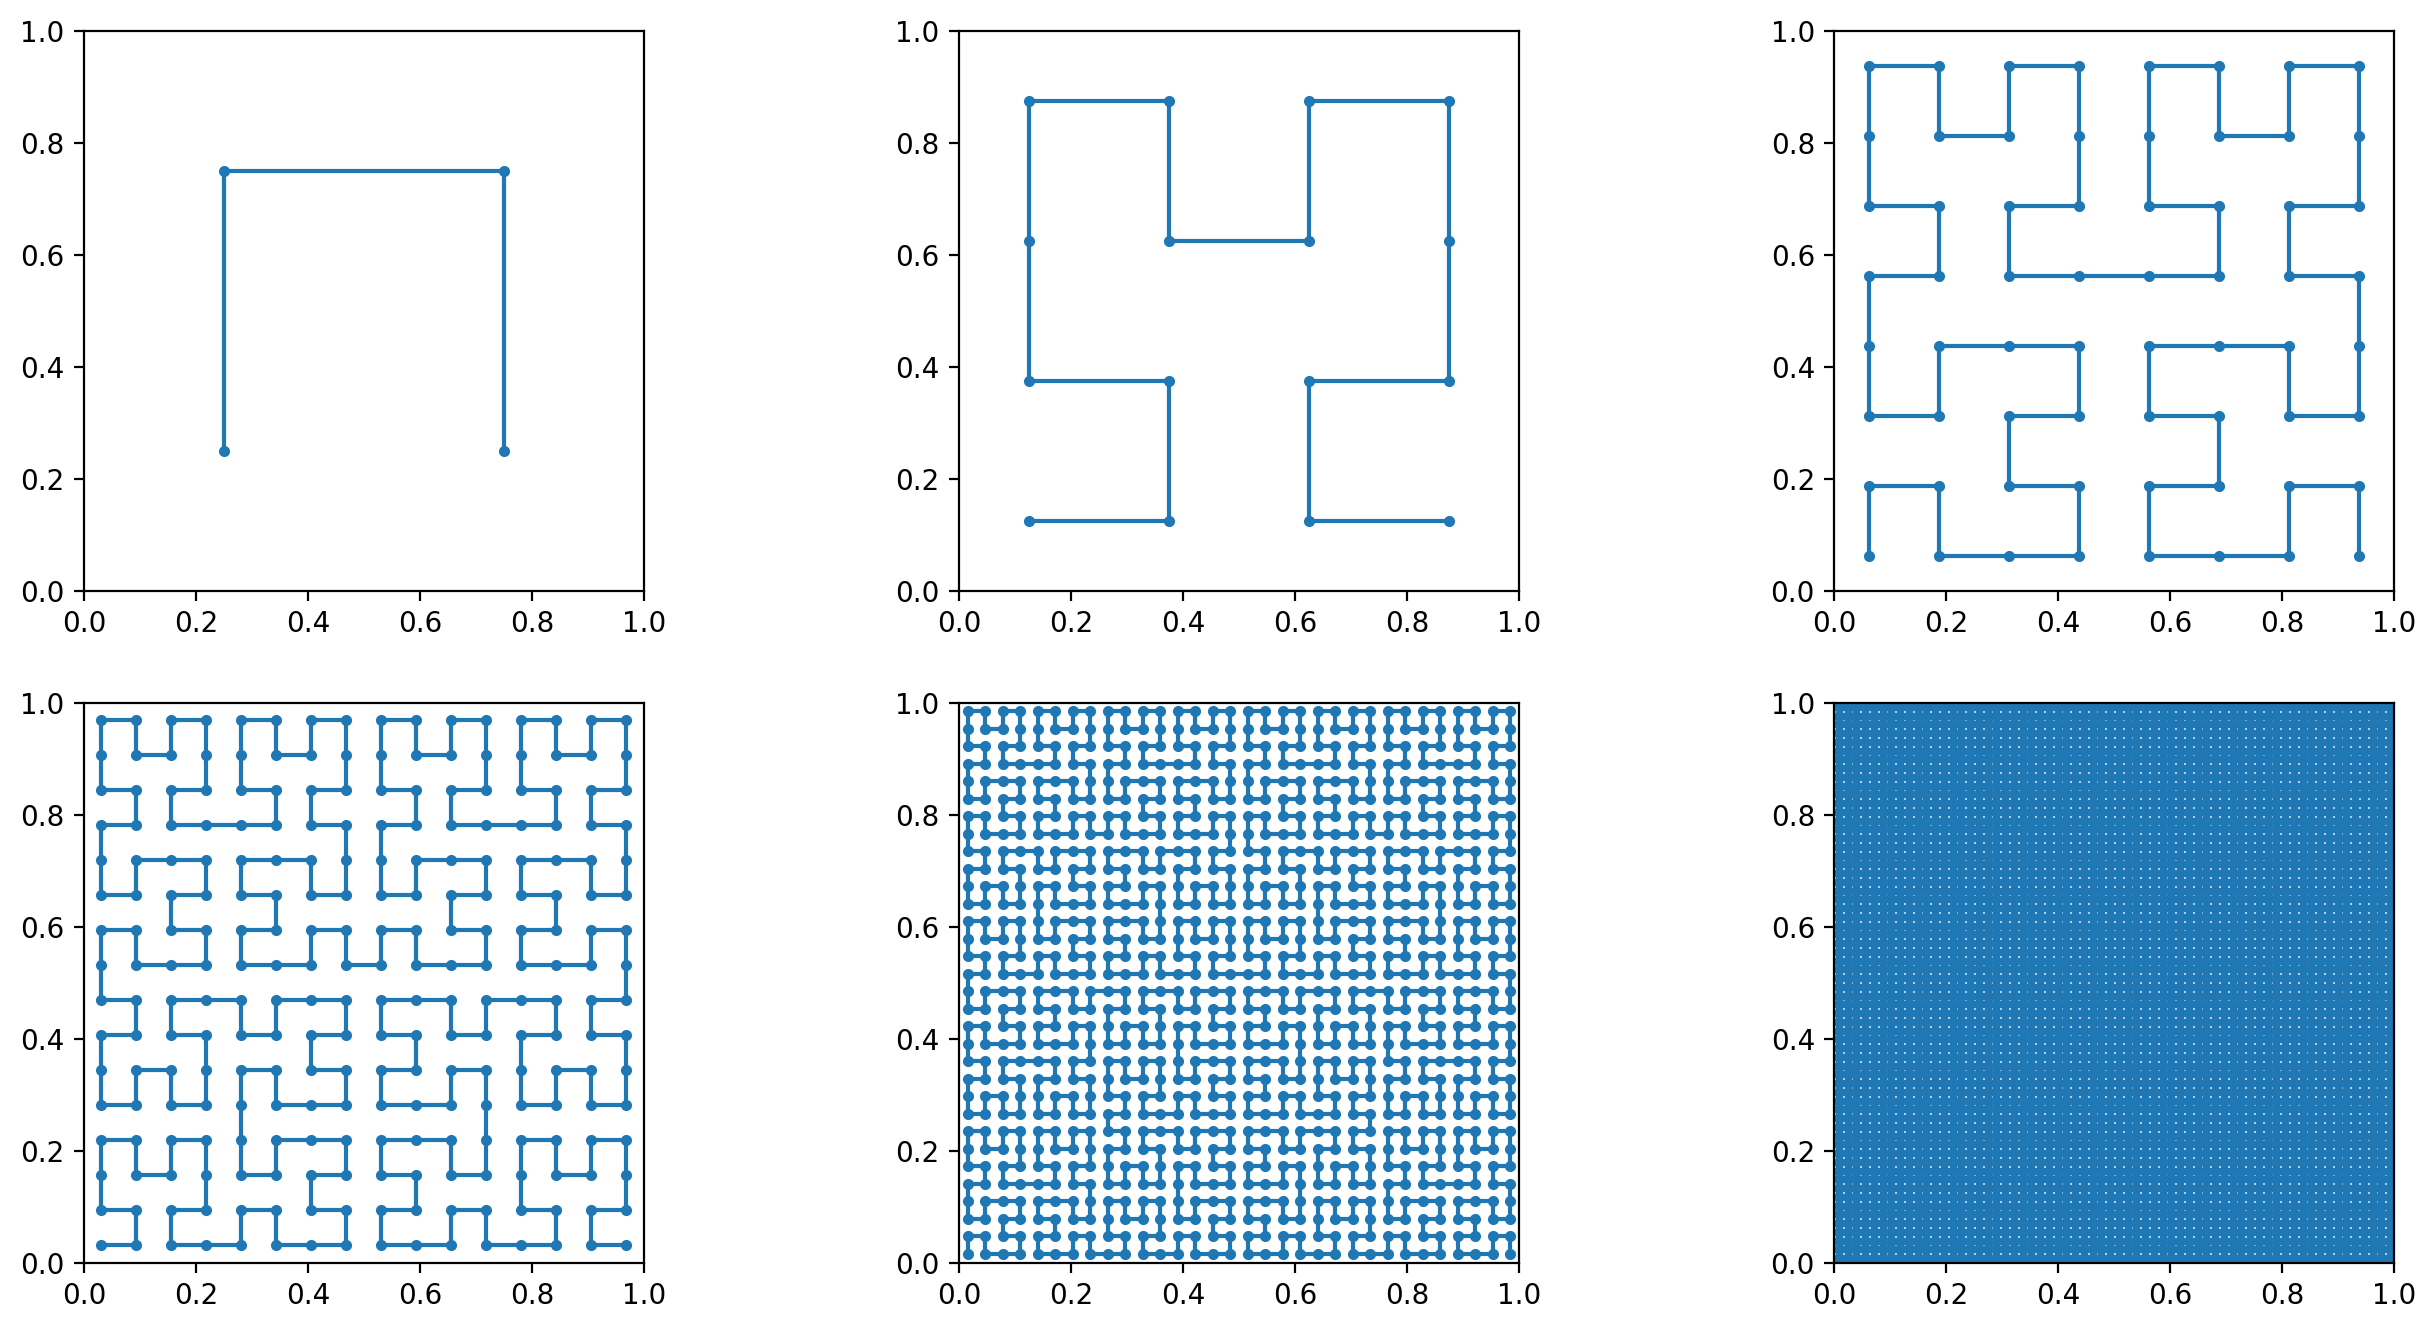
\includegraphics[width=0.99\textwidth]{figures/hilbertCurveFirstSixIterations.png}
    \caption{First six orders of the 2-dimensional approximate Hilbert curve, from $H_1$ to $H_6$.}
    \label{fig:hilbertCurveFirstSixIterations}
\end{figure}

Let $\mathcal{I}_m^{d}$ be the set of consecutive subintervals of $[0,1]$ of length $1 / 2^{d m}$,
\[
    \begin{aligned}
            \mathcal{I}_{m}^{d} & = \left\{ I_{m}^{d}(k), k = 0, 1, \ldots, 2^{dm} - 1\right\}\\
            &=  \left\{ \left[ \frac{k}{2^{dm}}, \frac{k+1}{2^{d m}} \right], k = 0, 1, \ldots, 2^{d m} - 1 \right\},
    \end{aligned}
\]
then we have that $\left\{ H_m\big( I_m^{d}(k) \big) \right\}$ is a sequence of subcubes of $[0,1]^{d}$ which have the following properties:
\begin{itemize}
    \item \label{item:bijection} (\textit{Bijection}): Each subinterval is mapped to a different section of the space,
        \[
                    H_m \big( I_{m}^{d}(k) \big) \neq  H_m \big( I_{m}^{d}(k') \big) \quad \text{for } k \neq  k'
        \]

    \item \label{item:adjacency} (\textit{Adjacency}): For any $k$, the two successive subcubes $H_m \big( I_{m}^{d}(k) \big)$ and $ H_m \big( I_{m}^{d}(k + 1) \big)$ have exactly a ($d-1$)-dimensional face in common.
        
    \item \label{item:nesting} (\textit{Nesting}): Increasing the curve order from $m$ to $m+1 $ corresponds to partitioning of each cube $H_m\big( I_m^{d}(k) \big)$ into $2^{d}$ subcubes.
        More specifically, for $k_{i} = 2^{d}k + i$, $i = 0, 1, \ldots, 2^{d} - 1$, the union of the $2^{d}$ successive subcubes $H_{m+1}\big( I_{m+1}^{d}(k_{i}) \big)$ yields the cube $H_{m}\big( I_{m}^{d}(k) \big)$.
\end{itemize}

In order to obtain a binary partition of $[0,1]^{d}$ at each scale $s$, we set $m = \left\lceil s / d \right\rceil $ and we join together every $2^{|d-s| \bmod d}$ subcubes.
This produces a valid dyadic partition by virtue of the bijection, adjacency, and nesting properties of the Hilbert curve.
Moreover, since successive subcubes are adjacent, we partition the subrectangles along the dimension that each pairwise group of $2^{|d-s| \bmod d}$ subcubes do not share.
\Cref{fig:partition-2d} shows the proposed binary partition scheme in the two-dimensional case.
Following the ordering of the centers of the approximate Hilbert curve, we obtain an ordering in the subrectangles of $[0,1]^{d}$.
At each fixed depth $s$, we can assign each subrectangle from left to right to the binary nodes in \Cref{fig:btree}.
This allows us to construct a binary tree partition of $[0,1]^{d}$ such that properties \eqref{eq:locationSpan} and \eqref{eq:locationSpanChildren} are both satisfied.

\begin{figure}[htbp]
    \centering
    % trim l b r u
    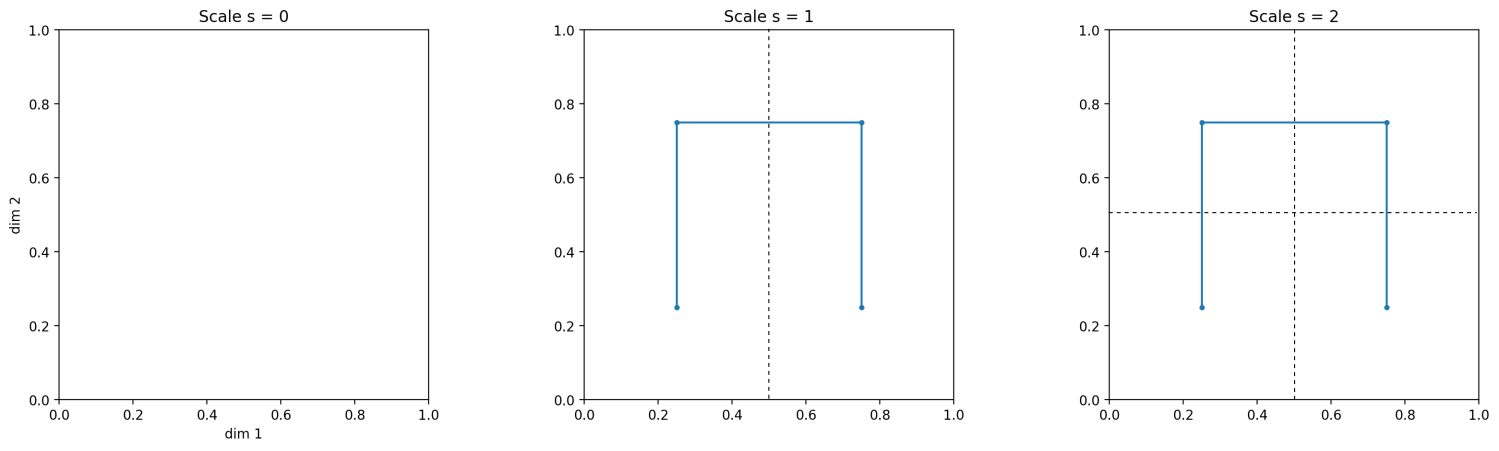
\includegraphics[trim={0 0 0 0}, clip, width=\textwidth]{figures/partition_2d_top2.png}
    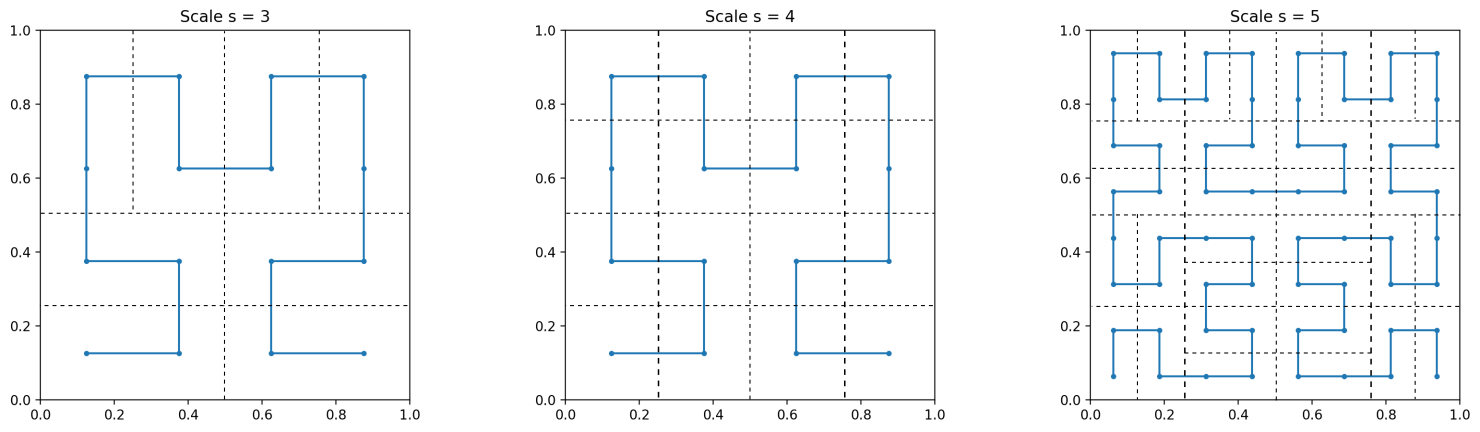
\includegraphics[trim={0 0 0 0}, clip, width=\textwidth]{figures/partition_2d_bot2.png}
    \caption{Dyadic partition of the two-dimensional square obtained by the application of the Hilbert curve, for the first six scales of the binary tree. 
    }
    \label{fig:partition-2d}
\end{figure}
% \subsection{Mixture of Gaussians}\label{sec:mixture-gaussians}

Let now $G_0$ be a base probability measure on $\Theta_{\bm{\mu}}$.
Once the space $[0,1]^{d}$ has been partitioned into subrectangles, we can obtain a suitable partition of $\R^{d}$ simply by applying the quantile function of each conditional distribution of $G_0$ to the extremes of the interval $[\bm{a}_{s,h}, \bm{b}_{s,h}]$, i.e.
\begin{equation}
    \label{eq:ThetaQuantiles}
    \Theta_{\mu^{(j)};s,h} = [q^{(j)}_{a^{(j)}_{s,h}}, q^{(j)}_{b^{(j)}_{s, h}}], \quad j = 1, \ldots, d,
\end{equation}
where $q^{(j)}(\cdot )$ is the conditional quantile function of $G_0$ for the $j$-th component.
Finally, we obtain the complete space partition by considering the Cartesian product
\[
    \Theta_{\bm{\mu}; s,h} = \Theta_{\mu^{(1)}; s,h}\times \Theta_{\mu^{(2)}; s,h} \times  \cdots \times \Theta_{\mu^{(d)}; s,h}.
\]

With this choice of partition, the locality property of the Hilbert curve ensures that nodes which are close on the binary tree refer to partitions which are close on $\R^{d}$.
This allows us to inspect the posterior distribution of the weights of the binary tree to infer the shape of the estimated multidimensional density.

We sample each location parameter $\bm{\mu}_{s,h}$ proportionally to $G_0$ truncated to the set $\Theta_{\bm{\mu};s,h}$,
so that the random probability measure
\begin{equation}
    \label{eq:randomLocationMeasure}
    G = \sum_{s=0}^{\infty }\sum_{h=1}^{2^s} \pi_{s,h} \delta_{\bm{\mu}_{s,h}}
\end{equation}
defined on $\Theta_{\bm{\mu}}$ is centered around $G_0$, as shown in \Cref{thm:centeringProperty}.

\begin{theorem}\label{thm:centeringProperty}
    Let $G_0$ be a base probability measure defined on $\Theta_{\bm{\mu}}$, and consider a dyadic partition of $\Theta_{\bm{\mu}}$ such as the one defined by Equations~\eqref{eq:locationSpan}, \eqref{eq:locationSpanChildren}, and \eqref{eq:ThetaQuantiles}.
    If $\bm{\mu}_{s,h}$ is randomly sampled proportionally to $G_0$ truncated to $\Theta_{\bm{\mu}; s,h}$, then, for any subset $A \subseteq \Theta_{\bm{\mu}}$,
    \begin{equation}
        \label{eq:priorCenteredMeasure}
        \mathbb{E}\big[ G(A) \big] = G_0(A).
    \end{equation}
\end{theorem}

\begin{proof}
    \[
        \begin{aligned}
            \mathbb{E}\big[ G(A) \big] & = \mathbb{E}\Big[  \sum_{s=0}^{\infty }\sum_{h=1}^{2^{s}}\pi_{s,h}\delta_{\bm{\mu}_{s,h}}(A) \Big]
\\
                                               &= \sum_{s=0}^{\infty } \sum_{h=1}^{2^{sz}}\mathbb{E}\big[ \pi_{s,h} \big] G_0(A \cap \Theta_{\bm{\mu};s,h})\\
                                               &= \sum_{s=0}^{\infty } \frac{(1-\delta) \prod_{j=0}^{s-1}(\alpha + \delta(j+1))}{\prod_{j=0}^{s}(\alpha+\delta j +1 )} \sum_{h=1}^{2^{s}} G_0(A \cap \Theta_{\bm{\mu};s,h})\\
                                               &= G_0(A) \sum_{s=0}^{\infty }\frac{(1-\delta) \prod_{j=0}^{s-1}(\alpha + \delta(j+1))}{\prod_{j=0}^{s}(\alpha+\delta j +1 )} \\
                                               &= G_0(A).
        \end{aligned}
    \]

\end{proof}



\section{Posterior computation}\label{sec:posterior-computation}
In this section we describe in detail the Markov Chain Monte Carlo algorithm we use to perform posterior inference for the multiscale model introduced in Section~\Cref{sec:msmk}.
The posterior computation for the multiscale stick-breaking mixture model is based on a blocked Gibbs sampler algorithm developed by \textcite{stefanucci2021}, where the kernels are assumed to be Gaussian for ease of derivation.
In this section, we also focus on the particular case of a Gaussian location-scale mixture of kernels, for which an extension of the aforementioned Gibbs sampler is straightforward.

Let $\pi_s = \sum_{h=1}^{2^{s}}\pi_{s,h}$ be the total probability mass assigned to scale $s$ and $\overbar{\pi}_{s,h} = \pi_{s,h} / \pi_s$ the proportion of mass associated to node $(s,h)$.
For the $i$-th observation we can rewrite the likelihood as
\[
    f(y_i) = \sum_{s=0}^{\infty }\pi_s \sum_{h=1}^{2^{s}} \overbar{\pi}_{s,h} \mathcal{K}(y_i; \vartheta_{s,h}).
\]
 Let now $(s_i, h_i)$ be auxiliary variables that indicate the node to which subject $i$ is allocated.
Conditionally on $s_i$ and $h_i$, we have that
\[
    f(y_i; s_i, h_i) \propto \mathcal{K}(y_i; \vartheta_{s_i, h_i}).
\]
Following \autocite{kalli2011}, we introduce an auxiliary random variable $u_i | y_i, s_i \sim \text{Unif}(0, \pi_{s_i})$, and write the joint density for $(y_i, u_i, s_i)$ as follows:
\[
    f(y_i, u_i, s_i) \propto \one_{(0, \pi_{s_i})}(u_i)  \sum_{h=1}^{2^{s_i}}\overbar{\pi}_{s_i, h} \mathcal{K}(y_i;\vartheta_{s_i, h_i}).
\]
Then, we can sample cluster indicators $s_i$ and $h_i$ by sampling from the following conditional distributions:
\begin{equation}
    \label{eq:gibbsSamplerUpdateClusterS}
    \mathbb{P}(s_i = s | u_i, y_i) \propto \one_{(u_i, 1)}(\pi_{s}) \sum_{h=1}^{2^{s}} \overbar{\pi}_{s,h} \mathcal{K}(y_i ; \vartheta_{s,h}),
\end{equation}
\begin{equation}
    \label{eq:gibbsSamplerUpdateClusterH}
    \mathbb{P}(h_i = h | u_i, y_i, s_i) \propto \overbar{\pi}_{s_i, h} \mathcal{K}(y_i; \vartheta_{s,h}).
\end{equation}

Conditionally on the sampled cluster indicators, the mixture weights are sampled from

\begin{equation}
    \label{eq:gibbsSamplerUpdateClusterSsh}
    S_{s,h} | - \sim \text{Beta}\big(1 - \delta + n_{s,h}, \alpha + \delta(s+1) + v_{s,h} - n_{s,h} \big),
\end{equation}
\begin{equation}
    \label{eq:gibbsSamplerUpdateClusterRsh}
    R_{s,h} | - \sim \text{Beta}\big(\beta +  r_{s,h}, \beta + v_{s,h} - n_{s,h} - r_{s,h} \big).
\end{equation}
Where $n_{s,h}$ is the number of subjects allocated to node $(s,h)$, $r_{s,h}$ is the number of subjects that continue to the right after passing through node $(s,h)$, and $v_{s,h}$ is the number of subject passing through node $(s,h)$ \autocite{canale2016b}.
Conditionally on cluster allocations, the update of kernel parameters depends on model specification.
In this section, we propose two versions of the MSM of Gaussian densities, namely the \textit{product kernel} and the \textit{full-covariance kernel}.
Whereas the former assumes a diagonal covariance matrix $\Omega_{s,h} = \diag \big( \omega_{s,h}^{(j,j)} \big)$  for the Gaussian kernel, the latter allows a full covariance matrix.

\subsection{Product kernel}\label{ssec:product-kernel}
Under the product kernel specification, we sample each component of the location parameter from
\begin{equation}\label{eq:gibbsSamplerIndepMean}
    \mu_{s,h}^{(j)} | - \sim N_{\Theta_{\mu^{(j)}; s,h}} \left(\frac{\mu_0\omega^{(j, j)}_{s,h} + n_{s,h}\bar{y}^{(j)}_{s,h}\kappa^{(j)}}{n_{s,h}\kappa^{(j)} + \omega^{(j)}_{s,h}}, \frac{\omega^{(j,j)}_{s,h}\kappa^{(j)}}{n_{s,h}\kappa^{(j)} + \omega^{(j,j)}_{s,h}}\right).
\end{equation}
where $\overbar{y}_{s,h} = \big( \overbar{y}^{(1)}_{s,h}, \overbar{y}^{(2)}_{s,h}, \ldots, \overbar{y}^{(d)}_{s,h} \big)$ is the sample mean of the observations assigned to node $(s,h)$, and $N_{A}(m,v)$ denotes the Gaussian distribution with mean $m$ and variance $v$ truncated to the set $A$.
Similarly, we update the scale parameters by sampling from
\begin{equation}
    \label{eq:gibbsSamplerIndepScale}
    \omega_{s,h}^{(j, j)} | - \sim \text{IGa}\bigg( k + \frac{n_{s,h}}{2}, \frac{\lambda}{2^{s}} + \frac{\sum_{i : s_i = s, h_i=h}(y_i^{(j)} - \mu_{s,h}^{(j)})^2 }{2}  \bigg).
\end{equation}

This specification of the multiscale model is simply an application of the original univariate multiscale model in \autocite{stefanucci2021} to each coordinate independently.

\subsection{Full-covariance kernel}\label{ssec:full-covariance-kernel}
Under the full-covariance kernel specification, the application of conjugate Bayesian analysis yields straightforward update rules.
More specifically, by assuming base measures $G_0 = MVN(\bm{\mu}_0, \Sigma_0)$ and $H_0 = \mathcal{IW}(\nu_0, \Psi)$ we sample the posterior scale parameters from
\[
    \Omega_{s,h} | - \sim \mathcal{IW}\bigg(\nu_0 + n_{s,h} + 2^{s}, \Psi + \sum_{i :\ \substack{s_i = s,\\h_i = h}} (y_i - \bm{\mu}_{s,h})(y_i - \bm{\mu}_{s,h})\tran \bigg),
\]
and the location parameters from
\[
    \bm{\mu}_{s,h} \sim \text{MVN}_{\Theta_{\bm{\mu};s,h}}\left( \bm{m}_{s,h}, \Sigma_{s,h} \right),
\]
where $\text{MVN}_A(\bm{m}, \Sigma)$ denotes the multivariate normal distribution of mean $\bm{m}$ and variance-covariance matrix $\Sigma$ truncated to the set $A$, and
\[
    \begin{aligned}
        \bm{m}_{s,h} & = (\Sigma_0^{-1} + n_{s,h}\Omega_{s,h}^{-1} )^{-1} (\Sigma_0^{-1} \mu_0 + n_{s,h}\Omega_{s,h}^{-1} \overbar{y}_{s,h}),\\
        \Sigma_{s,h} &= (\Sigma_0^{-1} + n_{s,h} \Omega_{s,h}^{-1})^{-1}.
    \end{aligned}
\]


\section{Simulation study}\label{sec:application}
In this section we conduct a simulation study to investigate the performance of the proposed multiscale model with respect to the known underlying distribution.
Moreover, we compare the multiscale method against its Bayesian nonparametric single-scale counterpart, the Pitman-Yor (PY) model \autocite{pitman1997}.
We generate samples $i = 1, \ldots, N$ with different sample sizes $n$ from different true distributions, which are obtained as mixtures of multidimensional normal and skew-normal distributions.
\autoref{fig:simulationCases} shows a two-dimensional representation of the considered scenarios, which present an increasingly evident multiscale structure.
\ldots

% \subsection{Synthetic data}\label{ssec:synthetic-data}

% \subsection{Sloan Digital Sky Survey data}\label{ssec:real-data}



\section{Discussion}\label{sec:discussion}
In this article we generalized the multiscale stick-breaking mixture model introduced by \textcite{stefanucci2021} to the multivariate setting.
This generalization retains the original binary-tree structure even when considering $d$-dimensional kernels for which $d \ge  2$.
We were able to do so by exploiting the ordering induced onto the $d$-dimensional space induced by the Hilbert curve in order to traverse the partitions of the location space $\Theta_{\bm{\mu}}$ by means of a binary tree.
This allowed us to straightforwardly generalize the Gibbs sampler algorithm via conjugate arguments in the multivariate Gaussian specification of the multiscale model.
When compared to a standard single-scale Bayesian nonparametric competitor such as the Pitman-Yor process, our proposed multiscale model showed competitive performance in terms of the LPML criterion, when equipped with a full-covariance kernel, especially when the density displayed an evident multiscale structure.

\printbibliography
\end{document}
